\chapter{Evaluierung}
\label{chapter:evaluierung}

Die Kapitel zuvor wurden die Streaming Frameworks Apache Storm, Apache Kafka, Apache Flume und Apache S4 vorgestellt eine Systemarchitektur für die einzelnen Prototypen definiert und die Implementierungen der Prototypen dokumentiert. In diesem Kapitel wird die Messung durchgeführt. Zuerst wird die Messumgebung beschrieben, anschließend wird jeweils zu den Prototypen eine Messung durchgeführt und das Messergebnis dargestellt. Weiterhin werden die Messergebnisse diskutiert und bewertet. Im Kapitel \ref{sec:diskussionUndBewertung} wird eine Erkenntnis aus der Bewertung gezogen und im letzten Kapitel wird eine Zusammenfassung gegeben.

\section{Messumgebung}
\label{sec:aufbauMessumgebung}

Die Messumgebung besteht wie im Kapitel \ref{chapter:systemarchitekur} Abbildung \ref{fig:useCaseMussKriterien} gezeigt aus zwei Maschinen für die Prototypen, einer virtuellen Maschine für die Verteilung der Log-Informationen und der Darstellung der Metriken. Verbunden sind die einzelnen Maschinen mit einem Switch. Die Messung selbst wird in mehreren Schritten durchgeführt. Zuerst werden schrittweise die Prototypen auf der High-End-Maschine \ref{tab:hiendwork} ausgeführt. Auf der Low-End-Maschine \ref{tab:loendwork} wird die virtuelle Maschine gestartet. Abschließend werden die Maschinen getauscht und auf der High-End-Maschine wird die virtuelle Maschine gestartet und auf der Low-End-Maschine werden die Prototypen schrittweise ausgeführt. Die Ausführung der Prototypen wurden im Kapitel \ref{chapter:prototypeDocumentation} bereits vorgestellt und die notwendige Vorbereitung der Maschine beschrieben. In der folgenden Liste werden die Kommandos für eine klare Übersicht schrittweise aufgezählt. \\\\

\textbf{Ausführung der Dienste auf der virtuellen Maschine}

\begin{verbatim}
>node storm/server.js
>node kafka/server.js
>node flume/server.js
>node s4/server.js
\end{verbatim}



\textbf{Ausführung des Storm-Prototypen}

\begin{verbatim}
>deployInteger.sh
>deployWord.sh
\end{verbatim}

Anschließend muss über die Storm-Web-Oberfläche der Prototyp gestartet bzw. gestoppt werden.\\\\


\textbf{Ausführung des Kafka-Prototypen}

\begin{verbatim}
>./bin/kafka-server-start.sh config/server.properties
>./bin/startIntProducer.sh
>./bin/startIntConsumer.sh
>./bin/startWordProducer.sh
>./bin/startWordConsumer.sh
\end{verbatim}

Die Ausführung des Kafka-Prototypen kann mit dem gleichzeitigen drücken der Tastenkombination \texttt{\gls{glo:strg}} und \texttt{C} beendet werden.\\\\


\textbf{Ausführung des Flume-Prototypen}

\begin{verbatim}
>./startAgentInteger.sh
>./startAgentWord.sh
\end{verbatim}

Der Flume-Prototype kann ebenfalls mit der Tastenkombination \texttt{\gls{glo:strg}} und \texttt{C} beendet werden.\\\\


\textbf{Ausführung des S4-Prototypen}

\begin{verbatim}
>startIntConsumer.sh
>startIntProducer.sh
>startWordConsumer.sh
>startWordProducer.sh
\end{verbatim}

Im S4-Prototype wird die Anwendung ebenfalls über die Tastenkombination \texttt{\gls{glo:strg}} und \texttt{C} beendet.

Nach der Vorstellung des Messaufbaus und der schrittweisen Ausführung der Kommandos der Prototypen, werden im nächsten Kapitel die Messergebnisse nach der Ausführung vorgestellt und beschrieben.

\section{Benchmark Ergebnisse}
\label{sec:benchmarkErgebnisse}

Im Kapitel zuvor wurden in einer kurzen Übersicht die notwendigen Kommandos für die schrittweisen Ausführung der Prototypen aufgezählt. Dieses Kapitel zeigt die Messergebnisse in einem Diagramm. Das Diagramm zeigt auf der Y-Achse die Anzahl der Nachrichten und auf der X-Achse die Zeit in Sekunden. Für eine gleichmäßige Darstellung der Diagramme wurde die Skala auf der Y-Achse so angepasst, damit die eingetragenen Messergebnisse für den Betrachter unmittelbar sichtbar sind. In einer Legende werden die Messergebnissen aus den einzelnen Messungen eines Prototypen farblich getrennt aufgelistet. Für die Darstellung in der Legende wurden Abkürzungen der einzelnen Messungen eingeführt. Die Farben \textit{Rot} und \textit{Blau} beziehen sich auf die Abkürzung \texttt{Hi} und bezeichnen die High-End-Maschine. Die Farben \textit{Orange} und \textit{Grün} beziehen sich auf die Abkürzung \texttt{Lo} und bezeichnen die Low-End-Maschine. Die Abkürzungen \texttt{Sta} und \texttt{Dyn} bedeuten für \texttt{Sta} statisch und \texttt{Dyn} dynamisch. Dabei steht \texttt{Sta} für die Messung mit konstanter Wortlänge und die Abkürzung \texttt{Dyn} für die Messung mit variabler Wortlänge. Neben der Nachrichten pro Sekunde wird zeitgleich die Prozessorbelastung in Prozent gemessen. So wird pro Prototyp zusätzlich ein Diagramm mit der Prozessorbelastung vorgestellt. Das Diagramm zeigt auf der Y-Achse die Prozessorbelastung in Prozent und auf der X-Achse die Zeit in Sekunden an. Farblich werden die Messungen genauso wie in dem Diagramm für die Messung der Nachrichtenanzahl. Die aufgezeichneten Messergebnisse liegen in einzelnen Dateien im Anhang bereit und sind in den folgenden Diagrammen als Messpunkte überführt.

Um einen möglichen Flaschenhals in der Datenverarbeitung auszuschließen, wird die virtuelle Maschine neben den Prototypen ebenfalls auf die Performance untersucht. Im Anhang wird ein Diagramm in Abbildung \ref{fig:messungMaxNachrichten} für die Messung von Nachrichten pro Sekunde gezeigt. Dabei kann ein Mittelwert von etwa 4000 Nachrichten pro Sekunde abgeleitet werden. Da in der Übersichtsseite\footnote{Systemübersicht der Prototypen Abbildung \ref{fig:systemOverviewStart}} der Prototypen nur eine Nachricht pro Sekunde angezeigt werden und die darunterliegenden Broker weniger als 1000 Nachrichten pro Sekunde verarbeiten müssen, kann damit ein Flaschenhals für die beschriebene Messung aus Kapitel \ref{sec:aufbauMessumgebung} in der virtuellen Maschine  ausgeschlossen werden. 

Die Abbildungen \ref{fig:messungStormDurchsatz} und \ref{fig:messungStormCpu} zeigen die Messungen zum Apache Storm Prototypen. Im Vergleich zwischen der High- und Low-End-Maschine werden während der Berechnung der Worte bei der variablen Wortlänge mehr Nachrichten pro Sekunde verarbeitet. Die High-End-Maschine verarbeitet im Durchschnitt 0,81\e{6} variable Wortlängen pro Sekunde im Vergleich zur konstanten Wortlänge mit 0,73\e{6} Nachrichten pro Sekunde. Die Prozessorbelastung ist bei der variablen Wortlänge 10 Prozent höher und liegt bei 53 Prozent. Bei der Low-End-Maschine ist ein ähnliches Verhalten festzustellen. In der variablen werden durchschnittlich 0,55\e{6} Nachrichten pro Sekunde im Vergleich zur konstanten Wortlänge mit 0,51\e{6} Nachrichten pro Sekunde übertragen. 

Im Unterschied zur High-End-Maschine liegt die Prozessorbelastung bei der konstanten Wortlänge bei 80 Prozent und ist 16 Prozent höher als bei der variablen Wortlänge. Weiterhin gibt es Unterschiede bei der Prozessorbelastung der Low-End-Maschine mit Lastspitzen in der 4ten, 66ten und 151ten Sekunde. Im Unterschied dazu ist die Prozessorbelastung bei der High-End-Maschine nach dem Start der Messung gleichmäßig. Der signifikante Unterschied wird auf die unterschiedlichen Prozessoren bezogen und wird in dieser Arbeit nicht näher betrachtet. In der Storm-Dokumentation\footnote{Storm Dokumentation zum Benchmark \textit{one million message per second per node}: \url{https://storm.incubator.apache.org/about/scalable.html}} wird bei einem Test mit einem spezifischen Prozessor 1,0\e{6} Nachrichten pro Sekunde erreicht. Nähere Angaben zu einem Test werden nicht angegeben und die gemessenen Messewerte unter den beschriebenen Messbedingungen in dieser Arbeit weiter betrachtet. Weiterführende Betrachtungen werden hierzu im Kapitel \ref{sec:diskussionUndBewertung} gegeben.


\begin{figure}[!ht]
%STORM TRHOUGHPUT%
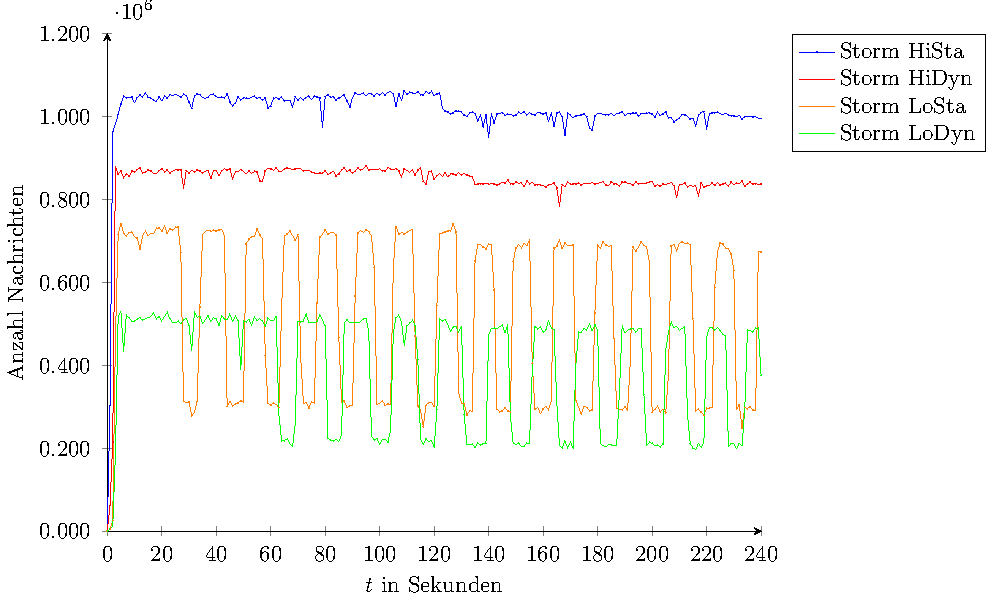
\includegraphics[width=0.97\textwidth]{plots/messungStormDurchsatz.pdf}
\caption{Messung Apache Storm Nachrichtendurchsatz
\label{fig:messungStormDurchsatz}}
%STORM CPU%
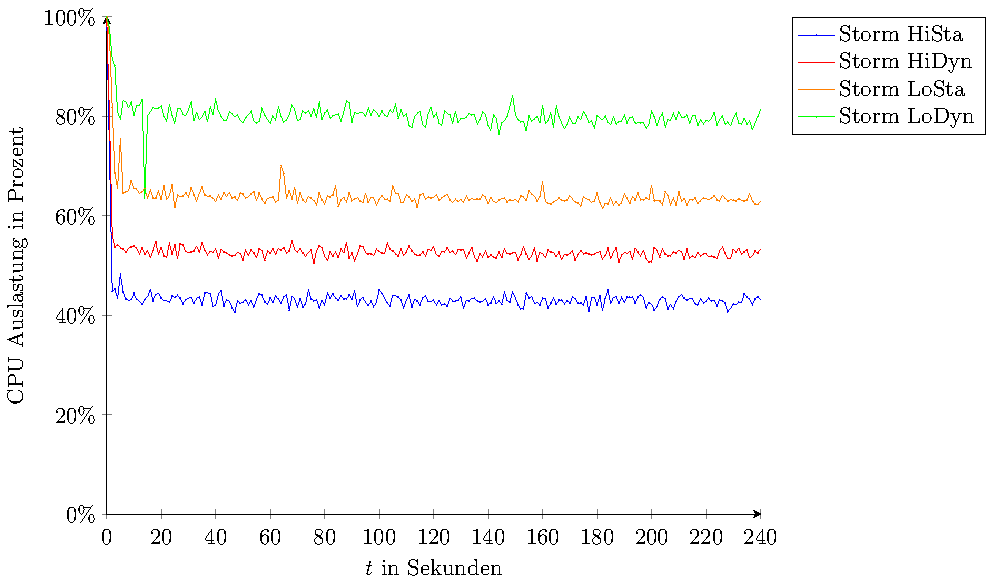
\includegraphics[width=0.97\textwidth]{plots/messungStormCpu.pdf}
\caption{Messung Apache Storm CPU Auslastung
\label{fig:messungStormCpu}}
\end{figure}


Die Abbildungen \ref{fig:messungKafkaNd} und \ref{fig:messungKafkaCpu} zeigen die Messergebnisse zum Apache Kafka Prototypen. Mit der High-End-Maschine werden im Durchschnitt 1,05\e{5} Nachrichten pro Sekunde in der Messung mit konstanter Wortlänge im Vergleich zur Messung der variablen Wortlänge im Durchschnitt mit 1,0\e{5} Nachrichten pro Sekunde übertragen. Die Prozessorbelastung ist bei der Messung mit konstanter Wortlänge im Durchschnitt 2 Prozent niedriger als bei der Messung mit variabler Wortlänge im Durchschnitt mit 41 Prozent. 


\begin{figure}[!ht]
%KAFKA TRHOUGHPUT%
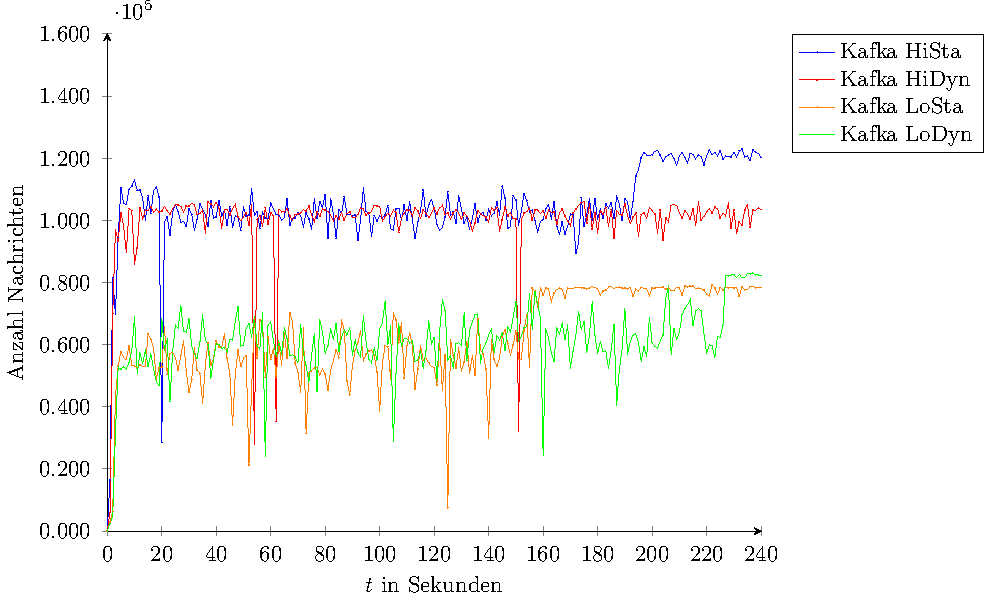
\includegraphics[width=0.97\textwidth]{plots/messungKafkaDurchsatz.pdf}
\caption{Messung Apache Kafka Nachrichtendurchsatz
\label{fig:messungKafkaNd}}
%KAFKA CPU%
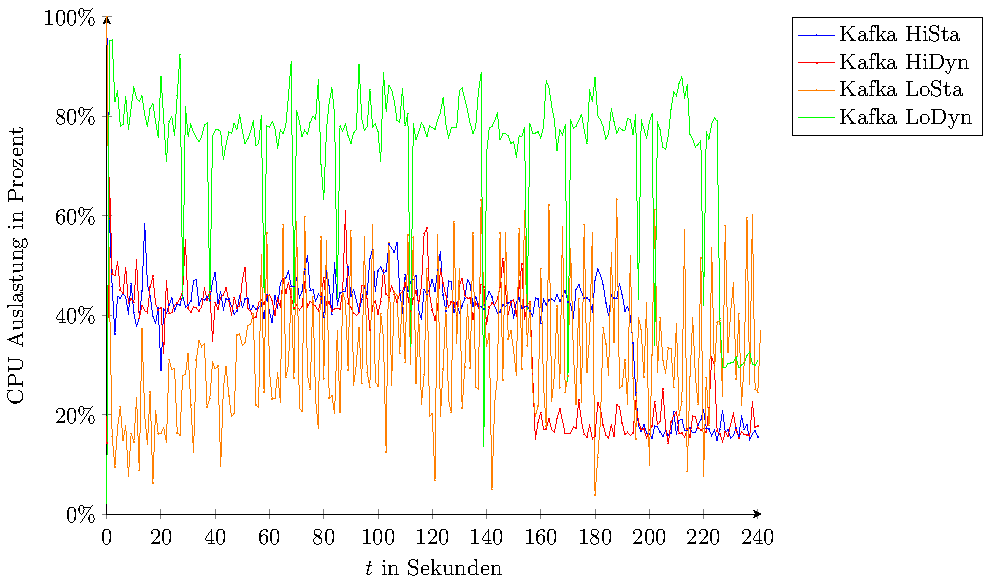
\includegraphics[width=0.97\textwidth]{plots/messungKafkaCpu.pdf}
\caption{Messung Apache Kafka CPU Auslastung
\label{fig:messungKafkaCpu}}
\end{figure}


Im Vergleich zur Low-End-Maschine verhält sich die Berechnung ähnlich. Es werden bei der Messung mit konstanter Wortlänge im Durchschnitt 0,62\e{5} Nachrichten pro Sekunde im Vergleich zur Messung der variablen Wortlänge mit 0,61\e{5} Nachrichten pro Sekunde im Durchschnitt übertragen. Der Unterschied der Prozessorbelastung ist in der Low-End-Maschine bei der Messung mit konstanter Wortlänge 19 Prozent niedriger als bei der Messung der variablen Wortlänge mit 71 Prozent. Weiterhin tauchen regelmäßige Lastspitzen in der Prozessorauslastung auf. Die höhere Last erklärt sich durch das Persistieren der Daten auf die Festplatte. Am Ende einer Messung in den variablen Wortlängen Variationen des Apache Kafka Prototypen wird der Prozessor massiv entlastet, da keine weiteren Daten aus einer Datei eingelesen werden. Der Apache Kafka \textit{Channel} arbeitet somit den Datenpuffer ab.


\begin{figure}[!ht]
%FLUME TRHOUGHPUT%
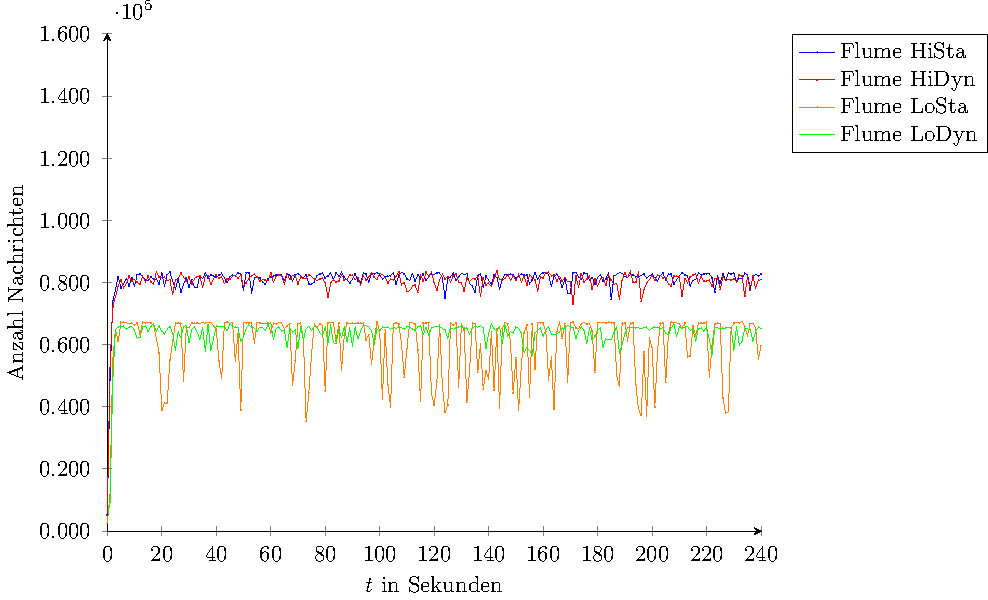
\includegraphics[width=0.97\textwidth]{plots/messungFlumeDurchsatz.pdf}
\caption{Messung Apache Flume Nachrichtendurchsatz
\label{fig:messungFlumeNd}}
%FLUME CPU%
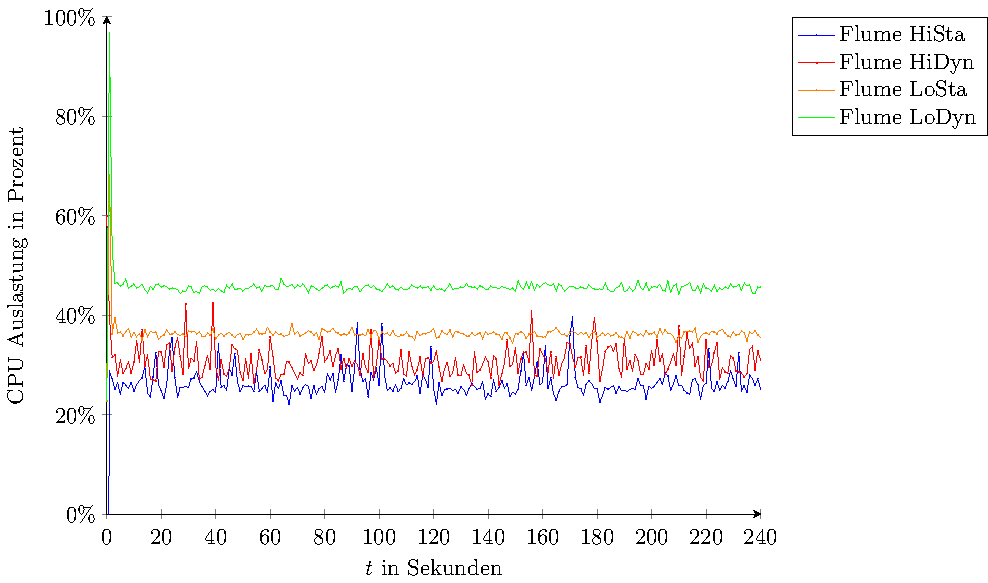
\includegraphics[width=0.97\textwidth]{plots/messungFlumeCpu.pdf}
\caption{Messung Apache Flume CPU Auslastung
\label{fig:messungFlumeCpu}}
\end{figure}


In Abbildung \ref{fig:messungFlumeNd} und \ref{fig:messungFlumeCpu} werden die Messungen zu dem Apache Flume Prototypen gezeigt. Die High-End-Maschine liefert bei der Messung mit konstanter Wortlänge im Durchschnitt 0,81\e{5} Nachrichten pro Sekunde und bei der Messung mit variabler Wortlänge im Durchschnitt 0,80\e{5} Nachrichten pro Sekunde. 

\begin{figure}[!ht]
%S4 TRHOUGHPUT%
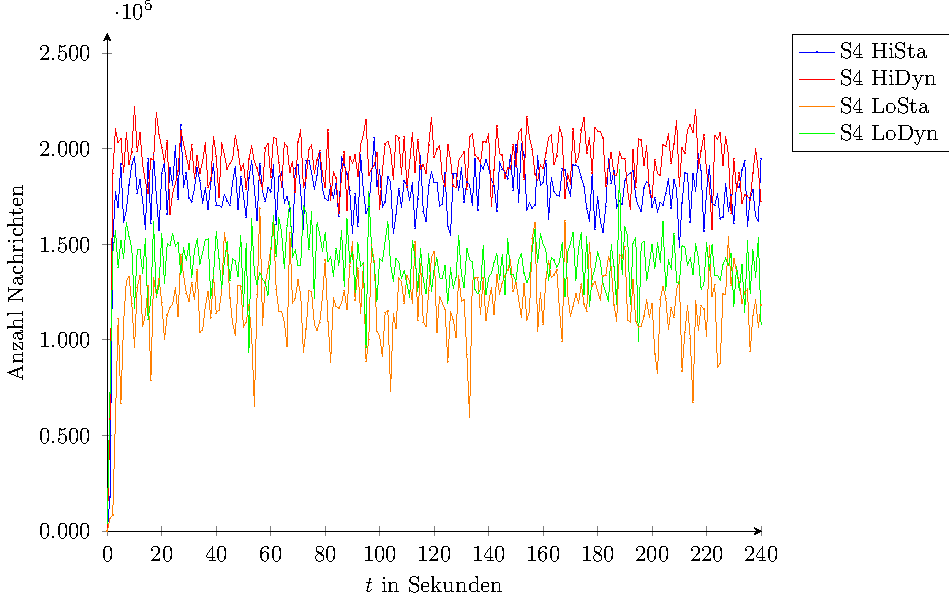
\includegraphics[width=0.97\textwidth]{plots/messungS4Durchsatz.pdf}
\caption{Messung Apache S4 Nachrichtendurchsatz
\label{fig:messungS4Nd}}
%S4 CPU%
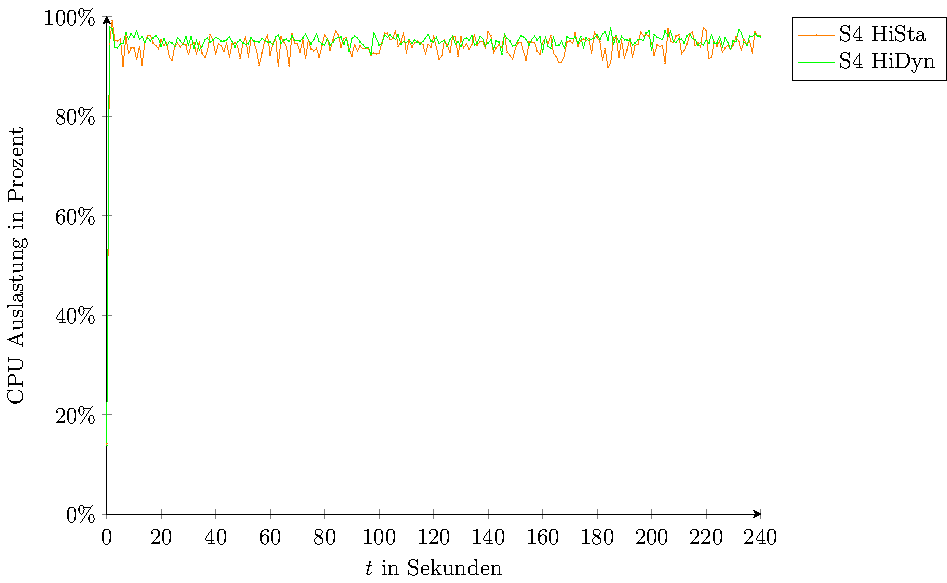
\includegraphics[width=0.97\textwidth]{plots/messungS4Cpu.pdf}
\caption{Messung Apache S4 CPU Auslastung
\label{fig:messungS4Cpu}}
\end{figure}

Dabei wird von der Messung mit konstanter Wortlänge im Durchschnitt 4 Prozent weniger Prozessorlast erzeugt, als bei der Messung mit variabler Wortlänge und der Prozessorlast von 24 Prozent. Bei nahezu gleicher Anzahl pro Sekunde wird von der Messung mit dynamischer Wortlänge mehr Prozessorlast benötigt. Die Low-End-Maschine verarbeitet im Durchschnitt in der Messung mit variabler Wortlänge im Durchschnitt 0,63\e{5} und mit konstanter Wortlänge im Durchschnitt 0,60\e{5} Nachrichten pro Sekunde. Die Prozessorlast liegt bei der Messung mit konstanter Wortlänge im Durchschnitt 10 Prozent niedriger und ist bei der Messung von variabler Wortlänge im Durchschnitt bei 43 Prozent. Im Vergleich zur High-End-Maschine wird bei der Low-End-Maschine mit der Messung der variablen Wortlänge im Durchschnitt mehr Nachrichten pro Sekunde bei erhöhter Prozessorbelastung übertragen.


Die Abbildungen \ref{fig:messungS4Nd} und \ref{fig:messungS4Cpu} zeigen die Messung des Apache S4 Prototypen. Mit den Messungen auf der High-End-Maschine werden bei der Messung mit konstanter Wortlänge im Durchschnitt 0,18\e{5} und bei der Messung mit variabler Wortlänge im Durchschnitt 0,19\e{5} Nachrichten pro Sekunde übertragen. Die Prozessorbelastung ist bei der Messung mit konstanter Wortlänge 57 Prozent und ist gegenüber der Messung mit variable Wortlänge im Durchschnitt 3 Prozent niedriger. Bei der Low-End-Maschine werden in der Messung mit konstanter Wortlänge im Durchschnitt 0,12\e{5} und mit variabler Wortlänge 0,14\e{5} Nachrichten übertragen. Die Prozessorbelastung liegt fast bei 100 Prozent. Die Messung mir konstanter Wortlänge beansprucht 93 Prozent und liegt 2 Prozent niedriger als die Messung mit variabler Wortlänge. Bei allen Varianten des Apache S4 Prototypen fallen viele Wechsel zwischen vielen und wenigen Nachrichten pro Sekunden in kleinen Zeitspannen gleichmäßig auf.

Nach der Beschreibung der Messergebnisse wird kurz auf die Darstellung der Übersichtsseite eingegangen. Mit der letzten Messung mit dem Prototypen Apache S4 wird die leere Übersichtsseite aus Abbildung \ref{fig:systemOverviewStart} durch den Broker mit Log-Informationen gefüllt. In der Abbildung \ref{fig:prototypeStreamingGraph} werden die Prototypen mit den Werten Nachrichten pro Sekunde und die ersten Fünf häufigsten Worten mit deren Anzahl gezeigt. Dabei wird farblich zwischen Gelb und Grün getrennt. Eine kleine Anzahl an Worten bekommt ein kräftiges Grün. Eine große Anzahl an Worten wird mit einem kräftigen Gelb in einem Balkendiagramm ausgegeben.


\begin{figure}[!ht]
\centering
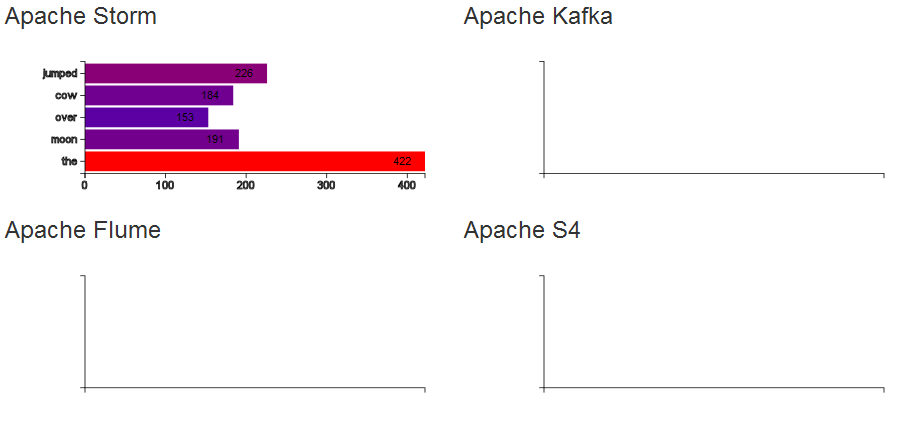
\includegraphics[width=1.0\textwidth]{bilder/PrototypeStreamingGraph.png}
\caption{Systemübersicht nach vollständiger Messreihe
\label{fig:prototypeStreamingGraph}}
\end{figure}


Nachdem in diesem Kapitel der Messaufbau vorgestellt, mehrere Messungen durchgeführt, die Ergebnisse dargestellt und erläutert wurden, werden im nächsten Kapitel die Ergebnisse vorgestellt, diskutiert und bewertet.


\section{Diskussion und Bewertung}
\label{sec:diskussionUndBewertung}

Im Kapitel \ref{sec:aufbauMessumgebung} und \ref{sec:benchmarkErgebnisse} wurden der Aufbau und die Struktur der Messung vorgestellt. Weiterhin wurden die Messungen durchgeführt, die Messergebnisse dargestellt und erläutert. In diesem Kapitel werden die gewonnen Ergebnisse zusammengetragen, diskutiert und bewertet.

In den Tabellen \ref{tab:avgSta} und \ref{tab:avgDyn} werden die Nachrichten pro Sekunde und die Prozessorbelastung in Prozent als Durchschnitte aus den Messergebnissen des Kapitels \ref{sec:benchmarkErgebnisse} aufgelistet. Aus den Durchschnitten kann ein Gesamtquotient aus den Messungen der konstanten und variablen Wortlängen und zwischen den High- und Low-End-Maschinen gezogen werden. Im Gesamtdurchschnitt wird der Prozessor der Low-End-Maschine etwa 24 Prozent mehr belastet und es werden etwa 31 Prozent weniger Nachrichten pro Sekunde, als mit der High-End-Maschine übertragen.

\begin{table}[!ht]
	\centering
		\begin{tabular}{@{}lrr@{}} \toprule
			\textbf{Streaming Framework} & \textbf{Nachrichtendurchsatz pro S} & \textbf{CPU Auslastung in \%} \\ \midrule
			Apache Storm Hi & 732003 & 43 \\
			Apache Storm Lo & 506703 & 80 \\
			Apache Kafka Hi & 104571 & 39 \\
			Apache Kafka Lo & 62423 & 52 \\
			Apache Flume Hi & 80953 & 20 \\
			Apache Flume Lo & 60095 & 33 \\
			Apache S4 Hi & 177036 & 57 \\
			Apache S4 Lo & 118507 & 93 \\
			\bottomrule			
		\end{tabular}
	\caption{Übersicht Durchschnitte Streaming Frameworks CPU Auslastung und Nachrichtendurchsatz bei konstanter Wortlänge}
	\label{tab:avgSta}
\end{table}

\begin{table}[!ht]
	\centering
		\begin{tabular}{@{}lrr@{}} \toprule
			\textbf{Streaming Framework} & \textbf{Nachrichtendurchsatz pro S} & \textbf{CPU Auslastung in \%} \\ \midrule
			Apache Storm Hi & 810005 & 53 \\
			Apache Storm Lo & 546328 & 64 \\			
			Apache Kafka Hi & 100009 & 41 \\
			Apache Kafka Lo & 61345 & 71 \\
			Apache Flume Hi & 80311 & 24 \\
			Apache Flume Lo & 63659 & 43 \\
			Apache S4 Hi & 192865 & 60 \\
			Apache S4 Lo & 139642 & 95 \\
			\bottomrule			
		\end{tabular}
	\caption{Übersicht Durchschnitte Streaming Frameworks CPU Auslastung und Nachrichtendurchsatz bei variabler Wortlänge}
	\label{tab:avgDyn}
\end{table}

Weiterhin können die Messergebnisse aus den Tabellen \ref{tab:avgSta} und \ref{tab:avgDyn} innerhalb der Maschinen zwischen der Messung mit konstanter Wortlänge und variabler Wortlänge verglichen werden. Zuerst wird die High-End-Maschine betrachtet. Bei den Prototypen Apache Storm und Apache S4 werden in der Messung mit konstanter Wortlänge weniger Nachrichten pro Sekunde übertragen und es wird weniger Prozessorlast erzeugt, als bei der Messung mit variabler Wortlänge. Im Unterschied dazu werden bei den Prototypen Apache Kafka und Apache Flume bei der Messung mit konstanter Wortlänge mehr Nachrichten pro Sekunde übertragen und weniger Prozessorlast erzeugt, als bei der Messung mit variabler Wortlänge. Als nächstes wird die Low-End-Maschine betrachtet. Die Prototypen Apache Kafka und Apache S4 haben das gleiche Verhalten wie unter der High-End-Maschine. Die Prototypen Apache Storm und Apache Flume zeigen ein unterschiedliches Verhalten gegenüber der High-End-Maschine. Der Prototype Apache Storm überträgt in der Messung mit konstanter Wortlänge weniger Nachrichten pro Sekunde und belastet den Prozessor stärker, als in der Messung mit variablen Wortlänge. Im Unterschied zur High-End-Maschine wurde der Prozessor weniger belastet. Beim Apache Flume Prototype werden in der Messung mit konstanter Wortlänge weniger Nachrichten pro Sekunde übertragen und weniger Prozessorlast erzeugt, als in der Messung mit variabler Wortlänge. Daraus kann ein relative konstantes Verhalten der Prototypen Apache Kafka und Apache S4 über den Vergleich der High- und Low-End-Maschine abgeleitet werden.

Bei der Betrachtung der Prozessorbelastung zwischen der High- und Low-End-Maschine, wird der Prozessor bei der Low-End-Maschine von Apache Storm und Apache S4 stärker und von Apache Kafka und Apache Flume schwächer belastet. Die Belastung des Prozessors liegt im Durchschnitt bei 60 Prozent. Bei der High-End-Maschine wird ein ähnliches Verhalten bei der Prozessorbelastung festgestellt. Die Prototypen Apache Storm und Apache S4 belasten den Prozessor stärker und die Prototypen Apache Kafka und Apache Flume belasten den Prozessor schwächer. Die Belastung des Prozessor liegt hier im Durchschnitt bei 50 Prozent. Daraus kann für die Prototypen Apache Storm und Apache S4 eine stärkere Nutzung des Prozessors gegenüber den Prototypen Apache Kafka und Apache Flume gefolgert werden.

Die Betrachtung des Nachrichtendurchsatzes pro Sekunden wird bezogen auf die Prozessorbelastung getrennt. Betrachtet werden zuerst die Prototypen, die den Prozessor stärker beanspruchen. Der Prototype Apache Storm überträgt die höchste Anzahl von Nachrichten pro Sekunde mit einem Spitzenwert von 8,85\e{5} Nachrichten pro Sekunde. Der Prototype Apache S4 überträgt in einem Spitzenwert von 2,22\e{5} Nachrichten pro Sekunde. Im Durchschnitt verarbeitet Apache Storm dennoch etwa 76 Prozent mehr Nachrichten pro Sekunde als Apache S4. Als nächstes werden die Prototypen mit schwacher Belastung des Prozessors betrachtet. Der Prototype Apache Kafka überträgt im Spitzenwert 0,11\e{5} Nachrichten pro Sekunde gegenüber Apache Flume mit dem Spitzenwert 0,08\e{5} Nachrichten pro Sekunde. Im Durchschnitt überträgt Apache Kafka 13 Prozent Nachrichten pro Sekunde mehr als Apache Flume. Insgesamt überträgt Apache Storm signifikant mehr Nachrichten pro Sekunde im Durchschnitt als die Prototypen Apache Kafka, Apache Flume und Apache S4. Bei den Prototypen Apache Kafka und Apache Flume gibt es kleine signifikante Unterschiede. In der Low-End-Maschine werden von Apache Flume weniger Nachrichten in der Messung mit konstanter Wortlänge übertragen als von der High-End-Maschine. Apache S4 unterscheidet sich zu Apache Kafka und Apache Flume in der höheren Übertragung der Nachrichten pro Sekunde und der stärkeren Belastung des Prozessors. Aus der Erkenntnis ergibt sich eine Rangfolge, in der zuerst Apache Storm mit sehr gutem Ergebnis abschneidet. Anschließend kommen Apache Kafka mit einem guten, sowie Apache Flume und Apache S4 mit einem befriedigendem Ergebnis. Die Rangfolge der Streaming Frameworks in dieser Arbeit beginnt somit mit Apache Storm, setzt weiter fort mit Apache Kafka und Apache Flume und endet mit Apache S4.

Nach der Diskussion der Messergebnisse und der Bewertung der Apache Prototypen basierend auf den Ergebnissen aus Kapitel \ref{sec:benchmarkErgebnisse}, werden zusätzlich die Kriterien aus Kapitel \ref{sec:funktAnforderung}, \ref{sec:nichtFunktAnforderung} und \ref{sec:loesungsansatz} auf Einhaltung überprüft. Zuerst werden die funktionalen Anforderungen aus Kapitel \ref{sec:funktAnforderung} betrachtet.

Der Einsatz von Apache Maven wie in \textbf{M1} gefordert erweist sich in Apache Storm, Apache Kafka und Apache Flume als einfach integrierbar. Apache S4 benutzt zur eigenen Entwicklung nicht Apache Maven und hat damit den Umstand eine Paketierung in Apache Maven nachzubilden. Alle Prototypen sind für die Paketierung mit Apache Maven vorbereitet. Alle Implementierungen der Prototypen erfolgte in der Entwicklungssprache Java. Die Ausführungen der Prototypen wurden unter dem Betriebssystem Linux durchgeführt. Damit ist \textbf{M2} erfüllt. Für die Ausführung der Prototypen wurde eine Umgebung mit einem Single-Node-Cluster bereitgestellt. In Kapitel \ref{chapter:prototypeDocumentation} werden der \textit{Start} und der \textit{Stop} jedes Single-Node-Clusters der einzelnen Streaming Frameworks vorgestellt. Eine Installation und Bereitstellung eines Single-Node-Clusters wird im Anhang \ref{sec:storminstall}, \ref{section:kafkainstall}, \ref{section:flumeinstall} und \ref{sec:s4install} schrittweise erklärt. \textbf{M3} wird damit erfüllt. Die Implementierung von zwei Varianten eines Prototypen, einem mit konstanter Wortlänge \textbf{M4} und einem mit variablen Wortlänge \textbf{M5} werden im Kapitel \ref{chapter:prototypeDocumentation} beschrieben und somit erfüllt. Die Implementierungen der Prototypen Apache Storm, Apache Kafka und Apache Flume erfolgte aufgrund einer guten Dokumentation reibungslos. Dennoch wird eine Quelltext-Dokumentation des Streaming Frameworks während der Entwicklung benötigt. Da Apache S4 eine stark veraltete Dokumentation hat und der Quelltext sehr schwach dokumentiert ist, bleibt nur ein schrittweises Vorgehen der Implementierung, unter Einsatz der Streaming Framework Quelltextes aus der Apache-Versionsverwaltung\footnote{Apache S4 Mirror auf github: \url{https://github.com/apache/incubator-s4}}. Die Aufnahme der Log-Informationen \textbf{M6} und Darstellung auf einer Übersichtsseite \textbf{M7} werden ebenfalls erfüllt und werden in diesem Kapitel \ref{sec:benchmarkErgebnisse} gezeigt und diskutiert. Die erfassten Messergebnisse stehen als Datei im Anhang \ref{section:inhaltDvd} bereit. Damit sind alle Muss-Kriterien erfüllt.

Das Soll-Kriterium \textbf{S1} erwartet eine Ausführung der Prototypen auf verschiedenen Rechnersystemen. In Kapitel \ref{sec:systemspezifiaktion} werden zwei verschiedene Rechnersysteme vorgestellt und in Kapitel \ref{sec:benchmarkErgebnisse} die Ergebnisse in einem Diagramm dargestellt und erläutert. So ist \textbf{S1} erfüllt. In \textbf{S2} sollen die ersten Fünf Wörter mit der höchsten Anzahl aus einem offenen und frei zugänglichen Datensatz berechnet und automatisch angezeigt werden. Im Kapitel \ref{sec:prot:aufbauStruktur} bezogen auf den Systementwurf aus Kapitel \ref{sec:systementwurf} gezeigt und beschrieben, wie die gemessenen Werte über den Broker an die Übersichtsseite gelangen. Außerdem wird auf \textbf{S3} eingegangen und der Transport der Nachricht über Javascript-Trigger im Kapitel \ref{sec:prot:aufbauStruktur} erklärt. Damit werden \textbf{S2} und \textbf{S3} erfüllt. Allerdings werden die Kann-Kriterien \textbf{K1}, die Ausführung der Prototypen auf einem Multi-Node-Cluster und \textbf{K2}, die Ausführung der Prototypen auf einem proprietären Betriebssystem nicht erreicht. Die Abgrenzungskriterien \textbf{A1} prototypische Entwicklung und \textbf{A2} Serverseitige Absicherung wird wie in der Dokumentation der Implementierung der Prototypen in Kapitel \ref{chapter:prototypeDocumentation} gezeigt, vollständig eingehalten.

Die Nichtfunktionalen Kriterien werden, wie in dem Kapitel \ref{sec:systementwurf} Systementwurf und in der Implementierung der Prototypen mit der Variante der variablen Wortlänge in Kapitel \ref{sec:prot:storm}, \ref{sec:prot:kafka}, \ref{sec:prot:flume} und \ref{sec:prot:s4} gezeigt, erfüllt. Mögliche Probleme und Lösungsansätze wurden in Kapitel \ref{sec:loesungsansatz} vorgestellt und bei der Beschreibung des Algorithmus in Kapitel \ref{sec:algorithmus}, des Vorgehens in Kapitel \ref{sec:vorgehen} und in der Implementierung in Kapitel \ref{chapter:prototypeDocumentation} berücksichtigt. Beim Messverfahren in Kapitel \ref{sec:prot:aufbauStruktur} und im Benchmark in Kapitel \ref{sec:benchmarkErgebnisse} werden die Ergebnisse sichtbar. Damit werden die Lösungsansätze aus Kapitel \ref{sec:loesungsansatz} von den Prototypen unterstützt. In diesem Kapitel wurden die Ergebnisse diskutiert und bewertet. Weiterhin wurden Anforderungen an die Prototypen auf Einhaltung geprüft und die Umsetzung erläutert. Abschließend wird im nächsten Kapitel eine Zusammenfassung zu diesem Kapitel gegeben.


\section{Zusammenfassung}

Im Kapitel \ref{chapter:evaluierung} wurde eine Evaluierung der Streaming Frameworks Prototypen Apache Storm, Apache Kafka, Apache Flume und Apache S4 durchgeführt. Zuerst wurde der Aufbau der Messumgebung vorgestellt und die Ausführung der Prototypen in kurzen Schritten aufgelistet. Dabei wurde auf das Starten und Stoppen der Prototypen eingegangen. Anschließend wurden die Prototypen ausgeführt und die Ergebnisse in Diagrammen dargestellt. Auf die Struktur der Diagramme wurde kurz eingegangen und die Messwerte wurden in einen Bezug gebracht. Auf spezifische Eigenschaften während der Messung und Ausprägungen in den Diagrammen, wie zum Beispiel Lastspitzen wurde eingegangen und in den Zusammenhang gebracht. Zusätzlich wird kurz die Übersichtsseite mit den empfangenen Messwerten gezeigt und erklärt. Abschließend werden die Messwerte im Kapitel \ref{sec:diskussionUndBewertung} diskutiert und bewertet. Zuerst wird mit einer tabellarischen Übersicht ein Überblick über die Messwerte im Durchschnitt gegeben. Daraus werden verschiedene Betrachtungen zwischen den eingesetzten Maschinen und den unterschiedlichen Prototype-Varianten vorgestellt und gegenübergestellt. Die Diskussionen bauen aufeinander auf und führen die Betrachtungen zu einem Ergebnis. Es wird das Ergebnis in Form einer Rangfolge vorgestellt. Das Ergebnis der Rangfolge der in dieser Arbeit verglichenen Streaming Frameworks ist: Apache Storm, Apache Kafka, Apache Flume, Apache S4. Weiterhin werden funktionelle und nichtfunktionelle Anforderungen aus Kapitel \ref{chapter:systemarchitekur} auf Einhaltung geprüft und deren Umsetzung erläutert. Das nächste Kapitel schließt diese Arbeit mit einer Schlussbetrachtung ab und gibt einen Ausblick.